% This is LLNCS.DEM the demonstration file of
% the LaTeX macro package from Springer-Verlag
% for Lecture Notes in Computer Science,
% version 2.4 for LaTeX2e as of 16. April 2010
%
\documentclass{llncs}
%
\usepackage{makeidx}  % allows for indexgeneration
\usepackage{amssymb}
\usepackage{amsmath}
\usepackage{algorithmic,eqparbox,array}
\usepackage{algorithm}
\usepackage{graphicx}
\usepackage{listings}
\usepackage{color}

    \definecolor{listcomment}{rgb}{0.0,0.5,0.0}
    \definecolor{listkeyword}{rgb}{0.0,0.0,0.5}
    \definecolor{listnumbers}{gray}{0.65}
    \definecolor{listlightgray}{gray}{0.955}
    \definecolor{listwhite}{gray}{1.0}


%\floatname{algorithm}{Procedure}
\renewcommand{\algorithmicrequire}{\textbf{Input:}}
\renewcommand{\algorithmicensure}{\textbf{Output:}}
\renewcommand{\algorithmiccomment}[1]{\hfill\eqparbox{COMMENT}{// #1}}
%
\begin{document}
%
\frontmatter          % for the preliminaries
%

\mainmatter              % start of the contributions
%
\title{Diffeomorphic Directly Manipulated Free-Form Deformation Image Registration via Vector Field Flows}
%
\titlerunning{Diffeomorphic DMFFD Image Registration}  % abbreviated title (for running head)
%                                     also used for the TOC unless
%                                     \toctitle is used
%
\author{Nicholas J. Tustison\inst{1} \and Brian B. Avants\inst{2}}

\authorrunning{N. J. Tustison and B. B.  Avants} % abbreviated author list (for running head)
\institute{University of Virginia, Charlottesville VA 22903, USA,\\
\email{ntustison@virginia.edu}
\and
University of Pennsylvania,
Philadelphia PA  18104,USA,\\
\email{avants@picsl.upenn.edu}}

\maketitle              % typeset the title of the contribution

\begin{abstract}
Motivated by previous work \cite{tustison2009} and 
recent diffeomorphic image registration developments in which the 
characteristic velocity field is represented by spatiotemporal B-splines 
\cite{de-craene2011}, we present a diffeomorphic B-spline-based
image registration algorithm combining and extending these techniques.  
The advancements of the proposed framework
over previous work include a preconditioned gradient descent algorithm and 
potential weighting 
of the metric gradient permitting, among other things, enforcement of 
stationary boundary conditions.  In addition to
theoretical and practical discussions of our contribution, we also describe 
its parallelized implementation as open source in the Insight Toolkit and
perform an evaluation on publicly available brain data.
%\keywords{B-splines, DMFFD, diffeomorphisms, image registration, ITK}
\end{abstract}

\section{Introduction}
Significant algorithmic developments characterizing modern intensity-based
image registration research include the B-spline parameterized approach
(so called {\em free-form deformation}) with early contributions 
including \cite{szeliski1997,thevenaz1998,rueckert1999}.  Amongst the 
variant extensions, the 
{\em directly manipulated free-form deformation} approach  \cite{tustison2009} 
 addressed the hemstitching issue associated with steepest descent traversal of
problematic energy topographies during the course of optimization.
%caused by the distribution of the uniform 
%B-spline shape functions over the transformation domain 

Other important image registration research
reflected increased emphasis on topological transformation considerations
in modeling biological/physical systems where topology is 
consistent throughout the course of deformation or a 
homeomorphic relationship is assumed between image domains.
Methods such as LDDMM \cite{beg2005} optimize time-varying velocity field 
flows to yield diffeomorphic transformations.  Alternatively, the FFD 
variant reported in \cite{rueckert2006} enforced diffeomorphic transforms
by concatenating multiple FFD transforms, each of which is constrained
to describe a one-to-one mapping.  Another FFD registration
incorporated the recent log-Euclidean framework for enforcing diffeomorphic
transformations \cite{Modat2011}.
Recently, the work of 
\cite{de-craene2011} combined these registration concepts into a single
framework called {\em temporal free-form deformation} in which the 
time-varying velocity field characteristic of LDDMM-style algorithms
is modeled using a 4-D B-spline object (3-D + time).  Integration of 
the velocity field yields the mapping between parameterized time points.

In this work, we describe our extension to these methods.  Similar to 
\cite{de-craene2011}, we also use an $N$-D + time B-spline object to 
represent the characteristic velocity field.  However, we use the 
directly manipulated free-form deformation optimization formulation to improve 
convergence during the course of optimization.  This also facilitates
modeling temporal periodicity and
the enforcement of stationary boundaries consistent with diffeomorphic
transforms.
We also incorporate B-spline mesh multi-resolution capabilities
for increased control during registration progression.  
Most importantly, we also describe
the parallelized algorithmic implementation as open source available through the Insight Toolkit.%
\footnote{
http://www.itk.org/
}

We first describe the methodology by laying out a mathematical description 
of the various algorithmic elements coupled with implementation details
where appropriate.  This is followed by an evaluation on publicly available
brain data. 

\section{Methods: Formulae  and Implementation}

In this section, we explain the underlying theory focusing on
differences with previous work.  We first explain how B-spline
velocity fields can be used to produce diffeomorphisms through
numerical integration involving the B-spline basis functions. 
We then show how our previous work involving optimization in 
B-spline vector spaces \cite{tustison2009} can be used for
optimization of diffeomorphisms.  Additional insight is then
gleaned by illustrating correspondence between theory and 
implementation.

\subsection{B-spline velocity field transform}

Briefly, as with other diffeomorphic formulations based on vector flows, we
assume the diffeomorphism, $\phi$, is defined on the image domain, $\Omega$, 
with stationary boundaries such that $\phi( \partial \Omega) = \mathbf{Id}$.
$\phi$ is generated as the solution of the ordinary differential
equation 
\begin{align}
  \label{eq:ode}
  \frac{d\phi(\mathbf{x}, t)}{dt} = v(\phi(\mathbf{x}, t), t),\,\,\phi( \mathbf{x}, 0 ) = \mathbf{x}
\end{align}
where $v$ is a (potentially) time-dependent smooth field, $v : \Omega \times t 
\rightarrow \mathrm{R}^d$ parameterized by $t \in [0,1]$.  Diffeomorphic mappings
between parameterized time points $\{t_a,t_b\} \in [0,1]$ 
are obtained from  Eq. (\ref{eq:ode}) through integration of the transport
equation, viz.
\begin{align}
  \label{eq:integral}
\phi(\mathbf{x},t_b) &= \phi(\mathbf{x},t_a) + \int_{t_a}^{t_b} v(\phi(\mathbf{x}), t) dt.
\end{align}
In the case of 
$d$-dimensional registration, we can represent the time-dependent velocity field  
as a $(d + 1)$-dimensional B-spline object
\begin{align}
v(\mathbf{x}, t) = \sum_{i_1=1}^{X_1}\ldots\sum_{i_d=1}^{X_d}\sum_{i_t=1}^T v_{i_1,\ldots,i_d,i_t} B_{i_t}(t) \prod_{j=1}^d B_{i_j}(x_j)
\end{align}
where $v_{i_1,\ldots,i_d,i_t}$ is a $(d+1)$-dimensional control point lattice
characterizing the velocity field and $B(\cdot)$ are the univariate B-spline
basis functions separately modulating the solution in each parametric dimension.

Although various methods exist for solving Eqns. (\ref{eq:ode}) and (\ref{eq:integral}),
we use $4^{th}$-order Runge-Kutta, i.e.
\begin{align}
  \phi_{n+1} &= \phi_{n} + \frac{1}{6}\left( k_1 + 2k_2 + 2k_3 + k_4 \right) \\
  t_{n+1} &= t_{n} + \Delta t \\ 
  \phi_0 &= \phi(t_0) 
\end{align}
where
\begin{align}
  k_1 &= v\left( \phi_{n}, t_{n} \right)\Delta t \\
  k_2 &= v\left( \phi_{n} + \frac{k_1}{2}, t_{n} + \frac{\Delta t}{2} \right)\Delta t \\
  k_3 &= v\left( \phi_{n} + \frac{k_2}{2}, t_{n} + \frac{\Delta t}{2} \right)\Delta t \\
  k_4 &= v\left( \phi_{n} + k_3, t_{n} + \Delta t \right)\Delta t
\end{align}  
which provides a more stable and reliable alternative than other numerical
methods \cite{press1996}.


%Combining Eqns. (\ref{eq:ode}) and (\ref{eq:integral}) we obtain
%\begin{align}
%\phi(\mathbf{x},t_b) = \phi(\mathbf{x},t_a) + \int_{t_a}^{t_b} \left( \sum_{i_1=1}^{X_1}\ldots\sum_{i_d=1}^{X_d}\sum_{i_t=1}^T 
%    v_{i_1,\ldots,i_d,i_t} B_{i_t}(t)\prod_{j=1}^d B_{j}(x_j) \right) dt 
%\end{align}
%Moving the integral inside the summations
%\begin{align}
%\label{eq:velocityfield}
%\phi(\mathbf{x},t_b) = \phi(\mathbf{x},t_a) + \sum_{i_1=1}^{X_1}\ldots\sum_{i_d=1}^{X_d} 
%        \underbrace{\left( \sum_{i_t=1}^T v_{i_1,\ldots,i_d,i_t} \int_{t_a}^{t_b} B_{i_t}(t) dt \right)}_{\phi'_{i_1,\ldots,i_d}} \prod_{j=1}^d B_{i_j}(x_j) 
%\end{align}
%demonstrates the sole dependency on the B-spline basis functions in
%the temporal parametric dimension.  The integral is easily calculated
%as the B-spline basis functions are piecewise polynomials.
%Also, it is seen that the 
%quantity inside the parentheses comprises the $d$-dimensional 
%control point lattice defining the diffeomorphic mapping
%defined between time points $[t_a,t_b]$ obtained by 
%integration.  Furthermore, supposing the initial diffeomorphism,
%$\phi(\mathbf{x}, t_a)$, is similarly parameterized, i.e.
%\begin{align}
%  \phi(\mathbf{x}, t_a) = \sum_{i_1=1}^{X_1}\ldots\sum_{i_d=1}^{X_d} \phi^{t_a}_{i_1,\ldots,i_d}\prod_{j=1}^d B_{i_j}(x_j), 
%\end{align}
%the diffeomorphism at $t_b$ is obtained by simple addition of the two control point 
%lattices,
%\begin{align}
%\phi(\mathbf{x},t_b) = \sum_{i_1=1}^{X_1}\ldots\sum_{i_d=1}^{X_d} \left(\phi^{t_a}+
%\phi' \right)_{i_1,\ldots,i_d} \prod_{j=1}^d B_{i_j}(x_j).
%\end{align}

\subsection{Directly manipulated free-form deformation optimization of the B-spline velocity field}

In \cite{tustison2009} 
it was observed that optimization of FFD registration with gradient descent is 
intrinsically susceptible to problematic energy topographies.  However, a
well-understood preconditioned gradient was proposed based on the work 
described in \cite{tustison2006} which we denote as directly manipulated
free-form deformation (DMFFD) image registration.  This alternative demonstrates 
improved performance over the steepest descent equivalent \cite{tustison2009}.

Similarly, for the time-varying velocity field case we propose the following preconditioned gradient,
$\delta v_{i_1,\ldots,i_d,i_t}$, given the similarity metric, $\Pi$,%
\footnote
{
Current options include neighborhood cross correlation (CC), mutual information (MI), and
sum of squared differences (SSD).
}
\begin{align}
\label{eq:dmffd}
  \delta v_{i_1,\ldots,i_d,i_t} &= \left( \sum_{c=1}^{N_{\Omega} \times N_t} \left( \frac{\partial \Pi}{\partial \mathbf{x}} \right)_c B_{i_t}(t^c)\prod_{j=1}^d B_{i_j}(x_j^c)  \right. \nonumber \\
  &\cdot \left. \frac{B_{i_t}^2(t^c) \prod_{j=1}^d B_{i_j}^2 (x_j^c)} 
  {\sum_{k_1=1}^{r+1}\ldots\sum_{k_d=1}^{r+1} \sum_{k_t=1}^{r+1} B_{k_t}^2(t^c) 
  \prod_{j=1}^d B_{k_j}^2 (x_j^c)} \right) \nonumber \\
  &\cdot\left({\sum_{c=1}^{N_{\Omega}\times N_t}B_{i_t}^2(t^c) \prod_{j=1}^d B_{i_j}^2 (x_j^c)} \right) ^{-1}
\end{align}
which is a slight modification of Eqn. (21)
in \cite{tustison2009} which takes into account the temporal locations of the 
dense gradient field sampled in $t \in [0,1]$. $N_t$ and $N_\Omega$ are the number
of time point samples and the number of voxels in the reference image domain, respectively.
$r$ is the spline order in all dimensions%
\footnote{
In terms of implementation spline orders can be specified separately for each dimension but, for simplicity,
we only specify a single spline order.  
}
and $c$ indexes the spatio-temporal dense metric
gradient sample.

Additionally, in \cite{tustison2006} it was shown that one could associate each 
metric gradient sample, $\left( \frac{\partial \Pi}{\partial \mathbf{x}}\right)_c$ with a confidence
weighting.  Thus, in order to enforce stationary boundaries, we 
assign image boundary metric gradients a value of zero with a corresponding
large confidence value.  

%Combining DMFFD optimization with the B-spline velocity field transform discussed in
%the previous subsection, we outline the iterative routine for optimizing the 
%velocity field control points in Algorithm \ref{alg1}.

%\begin{algorithm}                    
%\caption{Gradient descent optimization of the B-spline velocity field}        
%\label{alg1}      
%\begin{algorithmic}[1]
%\REQUIRE images $\mathcal{I}$ and $\mathcal{J}$
%\REQUIRE  user-specified similarity metric $\Pi$ 
%\REQUIRE  velocity field mesh size and multiresolution schedule, $R$
%\REQUIRE  number of time point samples, $N_t$ (default: 4)
%\REQUIRE  spline order (default: 3)
%\REQUIRE  gradient step size, $\lambda$ (default: 0.25)
%\ENSURE velocity field control point lattice, $v$
%\STATE $v \gets \mathbf{0}$ \COMMENT{Initialize velocity field}
%\FOR{number of resolution levels} 
%\FOR{number of iterations for current level} 
%  \STATE $G \gets []$  \COMMENT{Initialize dense gradient storage array}
%\FOR{$t = 1 \to N_t$ } 
%  \STATE $t' \gets \frac{t-1}{N_t-1}$  \COMMENT{Scale time point to $[0,1]$}
%  \STATE $\mathcal{I}' \gets \mathcal{I} \circ \phi(\mathbf{x}, t')$  \COMMENT{Warp $\mathcal{I}$ to the current time point}
%  \STATE $\mathcal{J}' \gets \mathcal{J} \circ \phi^{-1}(\mathbf{x}, 1-t')$ \COMMENT{Warp $\mathcal{J}$ to the current time point}
%  \STATE $G[t] \gets \frac{\partial \Pi(\mathcal{I}',\mathcal{J}')}{\partial \mathbf{x}}$  \COMMENT{Store dense similarity metric gradient}
%\ENDFOR  
%  \STATE $\delta v \gets B(G)$ \COMMENT{Calculate velocity lattice gradient (Eqn. (\ref{eq:dmffd}))}
%  \STATE $v \gets v + \lambda\delta v$ \COMMENT{Take a step in the gradient direction}
%\ENDFOR  
%  \STATE $v \gets R(v)$         \COMMENT{Refine lattice based on schedule}
%%  \IF {converged}
%%    \RETURN $v$
%%  \ENDIF
%\ENDFOR  
%\end{algorithmic}
%\end{algorithm}

\subsection{Implementation}

As mentioned previously, the registration algorithm has been implemented 
and introduced into the
Insight Toolkit and consists of the following major classes: 
\begin{itemize}
  \item \verb#itk::TimeVaryingVelocityFieldIntegrationImageFilter# ---
Implementation of 
the Runge-Kutta integration.  Given a 
sampled velocity field derived from the control point lattice as 
input and the lower and upper integration limits, integration is performed 
in a multi-threaded fashion (since each point in the domain
can be integrated separately).  
  \item \verb#itk::TimeVaryingBSplineVelocityFieldTransform#:
Handles the mapping of geometric primitives
using the transform described in this work.  It is defined by the velocity field
control point lattice which is sampled prior to being integrated to yield the 
resulting displacement field.  
  \item \verb#itk::TimeVaryingBSplineVelocityFieldImageRegistrationMethod#: 
  Coordinates the optimization
  using gradient descent given an user-specified number of resolution levels, shrink
  factors, and smoothing choices.  
  \item \verb#itk::TimeVaryingBSplineVelocityFieldTransformParametersAdaptor#:
  Handles the decomposition of the B-spline mesh resolution during the multi-resolution optimization
  given a user-specified scheduling. 
  \item \verb#itk::BSplineScatteredDataPointSetToImageFilter#:
  Calculates the similarity metric gradient (cf. Eqn. \ref{eq:dmffd}) which takes as input the 
  dense similarity metric gradient and an optional weighting for each gradient sample.  As 
  described earlier, this permits enforcement of stationary physical boundaries. % by specifying a zero gradient on the boundaries and a large weighting. 
\end{itemize}

Access to the new ITK 
registration framework (including the B-spline velocity field transform) 
is facilitated
via the command line module \verb#antsRegistration# available both in ANTs%
\footnote{
http://www.picsl.upenn.edu/ANTs
}
and accompanied by a technical report offered through the Insight Journal
\cite{tustison2012}.%
\footnote{
http://hdl.handle.net/10380/3334
}
%The interested reader should consult \cite{tustison2012} for further details on 
%actual usage.

\section{LPBA40 Evaluation}

As a preliminary evaluation for our algorithm we used a portion 
of the approach of Klein et al. \cite{Klein2009} in which 
various open brain data sets were used to evaluate different
segmentation algorithms.  Specifically, we used the first 20 
subjects of the LPBA40 data
set \cite{shattuck2008}%
\footnote{
http://www.loni.ucla.edu/Atlases/LPBA40
}
publicly available from the Laboratory of Neuro Imaging at
the University of California, Los Angeles.  Preprocessing included
brain extraction using the provided masks and N4 bias correction
\cite{tustison2010}.  

%Batch processing was facilitated by the inclusion of the proposed
%method in the ANTs interface to the new Insight Toolkit registration
%framework called \verb#antsRegistration# which is detailed in 
%\cite{tustison2012}.  An active development version is found in 
%the ANTS Sourceforge repository.%
%\footnote{
%http://sourceforge.net/projects/advants/
%}

A portion of the batch script used to produce the registrations is 
found in Listing \ref{listing:script}.  Each image was histogram-
matched prior to application of an initial affine transform using
the Demons metric.  The resulting transform was composed with the
proposed work using a neighborhood cross correlation similarity metric
\cite{avants2008} of radius = 4.  A multi-resolution strategy was 
employed where the initial B-spline velocity field mesh size was 
$24\times24\times12\times1$ which was doubled at each level.  
Other registration parameters can be gleaned from the Listing \ref{listing:script}.
Batch processing was performed on the linux cluster at the 
University of Virginia with allocation of 4 nodes for each job
multi-threading purposes.  Each registration took approximately
3 hours.

\vspace{2mm}
\lstset{frame = htb,
        framerule = 0.25pt,
        float,
        fontadjust,
        backgroundcolor={\color{listlightgray}},
        basicstyle = {\ttfamily\scriptsize},
        keywordstyle = {\ttfamily\color{listkeyword}\textbf},
        identifierstyle = {\ttfamily},
        commentstyle = {\ttfamily\color{listcomment}\textit},
        stringstyle = {\ttfamily},
        showstringspaces = false,
        showtabs = false
        numbers = none,
        numbersep = 6pt,
        numberstyle={\ttfamily\color{listnumbers}},
        tabsize = 2,
        language=bash,
        floatplacement=!h,
        caption={Representative script used for the LPBA40 
        evaluation.},
        captionpos=b,
        label=listing:script
        }
\begin{lstlisting}
# Register the n4 corrected moving LPBA subject to the 
# n4 corrected fixed LPBA subject.

antsRegistration --dimensionality 3 \
                 --output ${prefix} \
                 --use-histogram-matching 1 \
                 --transform Affine[0.5] \                # affine stage
                 --metric Demons[${fixed_n4},${moving_n4},1,0,Regular,0.01] \ 
                 --iterations 100x100x100 \
                 --smoothing-sigmas 4.0x3.0x2.0 \
                 --shrink-factors 4x3x2 \
                 --transform tvdmffd[0.75,24x24x12x1,4] \ # tv dmffd stage
                 --metric CC[${fixed_n4},${moving_n4},1,4] \ 
                 --iterations 40x50x2 \
                 --smoothing-sigmas 1.0x0.5x0.0 \
                 --shrink-factors 3x2x1

# Apply the resulting transforms (affine + tvdmffd) to the 
# moving labels.
                   
antsApplyTransforms --dimensionality 3 \
                    --input ${moving_labels} \
                    --reference-image ${fixed_n4} \
                    --output ${moving_warped_labels} \
                    --n NearestNeighbor \
                    --transform ${prefix}1Warp.nii.gz \
                    --transform ${prefix}0Affine.mat \
                    --default-value 0
\end{lstlisting}

Registration assessment used the average target overlap 
\cite{tustison2009a} for each of the 56 LPBA40 labeled regions.
The numerical values of this assessment are given in Table 1.
These values were projected onto LBPA40 Subject 1 for display in Fig. 1
which can be compared to a similar display given in \cite{Klein2009}
with the caveat that the colormap is slightly different. 

\begin{figure}
\centering
\begin{tabular}{c}
  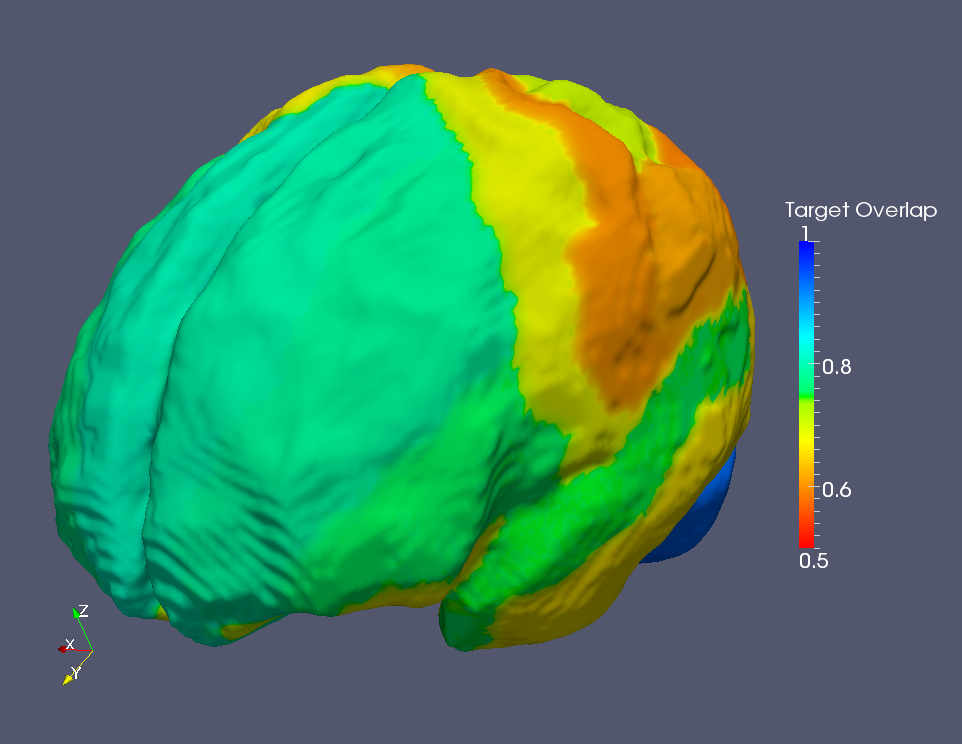
\includegraphics[width=120mm]{Figures/leftHemisphere.png} \\
  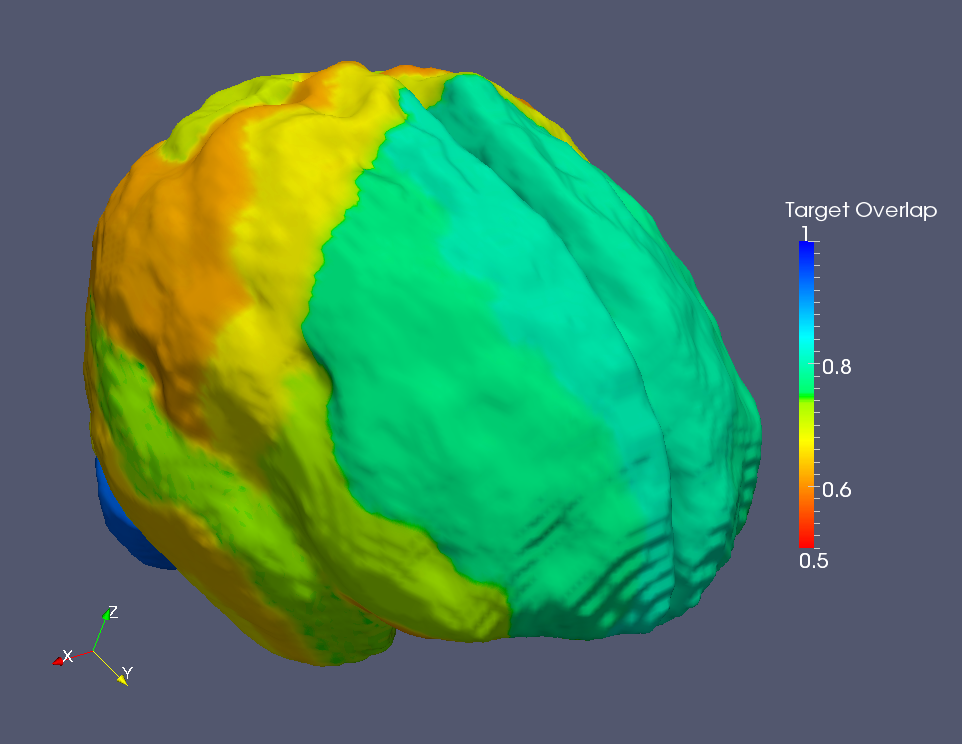
\includegraphics[width=120mm]{Figures/rightHemisphere.png}
\end{tabular}
\caption{Average regional total overlap measures mapped onto Subject 1
of the LPBA40 data set.}
\label{fig:lpba40}
\end{figure}

\setlength{\tabcolsep}{4pt}

\begin{table}[ht]
\begin{minipage}[b]{0.5\linewidth}\centering
\begin{tabular}{lc}
{\bf Region} & {\bf Overlap} \\
\hline
L superior frontal gyrus & 0.802 \\
R superior frontal gyrus & 0.810 \\
L middle frontal gyrus & 0.790 \\
R middle frontal gyrus & 0.778 \\
L inferior frontal gyrus & 0.753 \\
R inferior frontal gyrus & 0.728 \\
L precentral gyrus & 0.687 \\
R precentral gyrus & 0.674 \\
L middle orbitofrontal gyrus & 0.687 \\
R middle orbitofrontal gyrus & 0.671 \\
L lateral orbitofrontal gyrus & 0.669 \\
R lateral orbitofrontal gyrus & 0.607 \\
L gyrus rectus & 0.654 \\
R gyrus rectus & 0.652 \\
L postcentral gyrus & 0.604 \\
R postcentral gyrus & 0.620 \\
L superior parietal gyrus & 0.709 \\
R superior parietal gyrus & 0.701 \\
L supramarginal gyrus & 0.619 \\
R supramarginal gyrus & 0.623 \\
L angular gyrus & 0.594 \\
R angular gyrus & 0.620 \\
L precuneus & 0.668 \\
R precuneus & 0.659 \\
L superior occipital gyrus & 0.548 \\
R superior occipital gyrus & 0.561 \\
L middle occipital gyrus & 0.671 \\
R middle occipital gyrus & 0.696 \\
\hline
\end{tabular}
\end{minipage}
\begin{minipage}[b]{0.5\linewidth}
\centering
\begin{tabular}{lc}
{\bf Region} & {\bf Overlap} \\
\hline
L inferior occipital gyrus & 0.621 \\
R inferior occipital gyrus & 0.637 \\
L cuneus & 0.622 \\
R cuneus & 0.624 \\
L superior temporal gyrus & 0.750 \\
R superior temporal gyrus & 0.737 \\
L middle temporal gyrus & 0.660 \\
R middle temporal gyrus & 0.644 \\
L inferior temporal gyrus & 0.662 \\
R inferior temporal gyrus & 0.674 \\
L parahippocampal gyrus & 0.711 \\
R parahippocampal gyrus & 0.707 \\
L lingual gyrus & 0.694 \\
R lingual gyrus & 0.681 \\
L fusiform gyrus & 0.703 \\
R fusiform gyrus & 0.719 \\
L insular cortex & 0.812 \\
R insular cortex & 0.768 \\
L cingulate gyrus & 0.691 \\
R cingulate gyrus & 0.676 \\
L caudate & 0.704 \\
R caudate & 0.717 \\
L putamen & 0.773 \\
R putamen & 0.761 \\
L hippocampus & 0.753 \\
R hippocampus & 0.742 \\
cerebellum & 0.935 \\
brainstem & 0.899 \\
\hline
\end{tabular}
\end{minipage}
\vspace{1.0mm}
\caption{Average target overlap values for cross-registration of the first 
20 subjects of the LPBA40 data set.  A visual depiction of these values is
given in Figure \ref{fig:lpba40}.
}
\end{table}

\section{Discussion and Conclusions}
This work constitutes an advantageous combination of the continuous aspects of
B-splines with the diffeomorphic registration framework via vector field 
flows.  We incorporate
DMFFD optimization of the B-spline velocity field which facilitates 
convergence and permits enforcement of stationary boundary conditions.  
While not discussed, further advantages include incorporation of temporal 
periodicity in dealing with the possibility of multiple images describing
periodic motion (e.g. cardiac or pulmonary motion). A future publication 
will explore these possibilities in greater detail. 

\bibliographystyle{splncs03}
\bibliography{references}

\end{document}
